\documentclass[12pt]{article}

\usepackage[a4paper, total={7in, 10in}]{geometry}
\usepackage{booktabs}
\usepackage{tikz}
\usepackage{xcolor}
\usepackage{amsmath}
\usepackage{amssymb}
\usepackage[noend]{algpseudocode}
\usepackage{graphicx}
\usepackage{minted}
\usepackage[vlined,boxed,ruled]{algorithm2e}

\graphicspath{ {.} }


\begin{document}

\section*{Problem 1}

\begin{enumerate}
 \item \textcolor{blue}{$\Theta(n)=n$} \par
    \begin{tabular}{@{}ccc@{}}
    \hline
    \# of iterations & n  \\ \midrule
    0                & 0  \\
    1                & 1  \\
    2                & 2  \\
    3                & 3  \\
    4                & 4  \\ \bottomrule
    \end{tabular}
 \item \textcolor{blue}{$\Theta(n)=\lg(\lg n)$} \par
    \begin{tabular}{@{}cccc@{}}
    \hline
    \# of iterations & n        & $\lg(n)$ & $\lg(\lg(n))$ \\ \midrule
    0                & $2^1$    & 1         &  0              \\
    1                & $2^2$    & 2         &  1              \\
    2                & $2^4$    & 4         &  2              \\
    3                & $2^8$    & 8         &  3              \\
    4                & $2^{16}$ & 16        &  4              \\ \bottomrule
    \end{tabular}
 \item \textcolor{blue}{$\Theta(n)=4^{n}$} \par
    \begin{tabular}{@{}cccc@{}}
    \hline
    Tree level & \# of calls                   & Input number     \\ \midrule
     0         & $4^{0}$                       & $n$              \\
     1         & $4^{1}$                       & $n-1$            \\
     $\vdots$  & $\vdots$                      & $\vdots$         \\
     $n-2$     & $4^{n-87506055}3^{87506055-2}$& 2                \\
     $n-1$     & $4^{n-87506055}3^{87506055}$  & 1                \\ \bottomrule
    \end{tabular}\par
    $4^{n-87506055}3^{87506055}=\Theta(n) \implies 4^{n}=\Theta(n)$
 \item \textcolor{blue}{True.} \par
    Obviously $f+g$ itself belongs to the set $\Theta(f+g)$,\\
      $\implies (f+g)c_{2}\leq f+g \leq (f+g)c_{1}$, where $c_{1}$ and $c_{2}$ are positive constants.\\
      $\implies c_{2}\text{max}(f,g)\leq c_{2}(f+g)\leq f+g \leq c_{1}(f+g)\leq 2c_{1}\text{max}(f,g)$\\
      $\implies c_{2}\text{max}(f,g)\leq f+g \leq c_{1}'\text{max}(f,g)$, where $c_{1}'=2c_{1}$\\
      $\implies f+g=\Theta(\text{max}(f,g)).$
 \item \textcolor{blue}{True.} \par
    $f=O(i)$ and $g=O(j)$\\
    $\implies$ There are two positive constants such that $0 \leq f \leq c_{1}i$ and $0 \leq g \leq c_{2}j$.\\
    $\implies 0 \leq fg \leq c_{1}c_{2}ij$
    $\implies fg=O(ij)$.
 \item \textcolor{blue}{False.} \par
    If $f=2\lg n$ then $g=\lg n$\\
    $\implies 2^{f}=2^{2\lg n}=2^{\lg n^{2}}=n^2$\\
    On the other hand, $2^{g}=2^{\lg n}=n$\\
    $\implies 2^{f}=O(n^2)\neq O(n) = 2^{g}$
 \item \textcolor{blue}{True.} \par
    As shown in the left figure, the total area of the red rectangles is obviously smaller than
    that under the curve $1/x$(blue line) between $1<x<n$. Hence, we obtain the upper bound as follows:

    \begin{equation}
       \sum_{k=1}^{n}\dfrac{1}{k}<1+\int_{1}^{n} \dfrac{1}{x}dx=1+\log n
       \label{upper}
    \end{equation}

    Similarly, the lower bound can be obtained from the right figure:

    \begin{equation}
       \sum_{k=1}^{n}\dfrac{1}{k}>\int_{1}^{n+1} \dfrac{1}{x}dx=\log (n+1)
       \label{lower}
    \end{equation}

    Finally, since both lower and upper bounds have the asymptotic form $\log n$,
    we have $\displaystyle\sum_{k=1}^{n}\frac{1}{k}=\Theta(\lg n)$.

    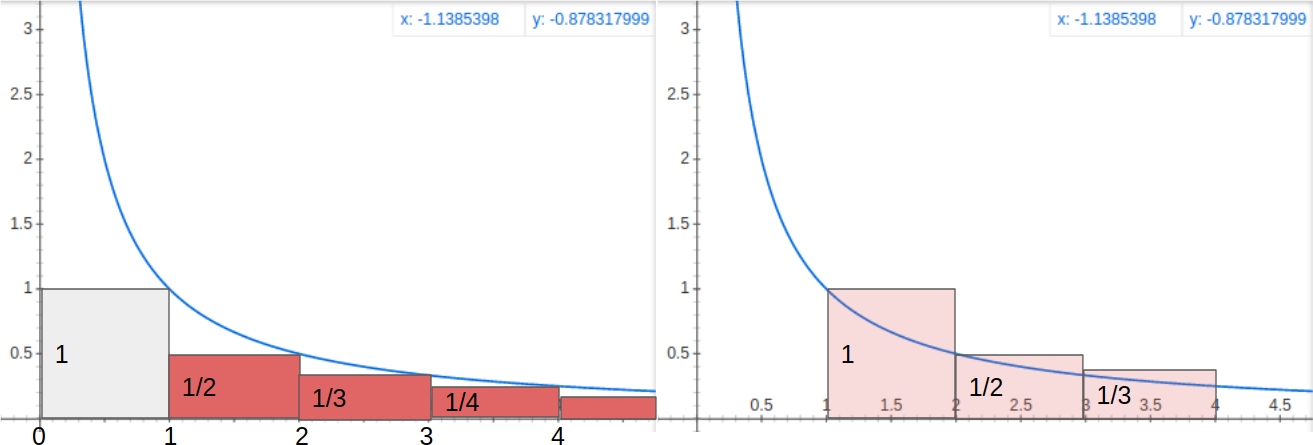
\includegraphics[scale=0.4]{c.png}
 \item \textcolor{blue}{True.} \par
    On the basis of approximation as follows:
    \begin{equation}
    \lg n! = \sum_{k=1}^{n} \lg k \sim \int_{1}^{n}\lg x dx=n\lg n-n+1,
    \end{equation}
    we have $\lg n! = \Theta(n\lg n)$.
 \item $\textcolor{blue}{f(n)=\Theta(n(\lg n)^2)}$.
    \begin{equation}
    \begin{aligned}
      f(n)&=2f\left(\frac{n}{2}\right)+n\lg n\\
          &=2\left[2f\left(\frac{n}{2^2}\right)+\frac{n}{2}\lg \left(\frac{n}{2}\right)\right]+n\lg n\\
          \vdots&\\
          &\sim\overbrace{2\times \dots \times 2}^{\sim\lg n \text{ times}}\times f(1)
             +\overbrace{(n\lg 1)+\dots+\left(n\lg \left(\frac{n}{2^2}\right)\right)+\left(n\lg \left(\frac{n}{2}\right)\right)+(n\lg n)}^{\sim\lg n \text{ times}}\\
          &\sim 2^{\lg n}+n\lg\left(\frac{n^{\lg n}}{2^{\lg n+\dots+2+1}}\right)\\
          &\sim n+n(\lg n)^2 - n \lg\left(2^{\lg n \times (\lg n+1)/2}\right)\\
          &\sim n+n(\lg n)^2 - n \left[ 0.5\lg n \left(\lg n +1\right) \right]\\
          &\sim n + 0.5n(\lg n)^2 -0.5n\lg n.
    \end{aligned}
    \end{equation}
Hence, $f(n)=\Theta(n(\lg n)^2)$.


\end{enumerate}

\section*{Problem 2}

\begin{enumerate}
  \item
    Reverse queue with another empty queue\par
    \begin{minipage}{.7\linewidth}
    \begin{algorithm}[H]
       \SetKwFunction{KwGetSize}{GetSize}
       \SetKwFunction{KwInitQueue}{InitQueue}
       \SetKwFunction{KwDeQueue}{DeQueue}
       \SetKwFunction{KwEnQueue}{EnQueue}

       \KwIn{1,2,3,4,5}
       \KwOut{5,4,3,2,1}
        Q1 = \KwInitQueue(1,2,3,4,5)\;
        Q2 = \KwInitQueue()\;

        \While{\KwGetSize{Q1} is greater than zero}
        {
          \While{the last element is at the front of Q1}
          {
               Q1 = \KwEnQueue{\KwDeQueue{Q1}}\;
          }
          Q2 = \KwEnQueue{\KwDeQueue{Q1}}\;
        }
    \end{algorithm}
    \end{minipage}
  \item 
    The number of iterations of outer loop: the size of initial queue, $n$.\\
    The number of iterations of inner loop: $n-k$, where $k$ is the \# of iterations of the outer loop at $k\text{-th}$ times.\\
    Hence, the time complexity is $n+(n-1)+\dots+1=0.5n(n+1)=O(n^2)-\text{time}$.\\
    We do not use the additional third array or queue to reverse queue. Thus extra-space complexity is $O(1)$.
  \item Illustration\par 


\tikzset{every picture/.style={line width=0.75pt}} %set default line width to 0.75pt        

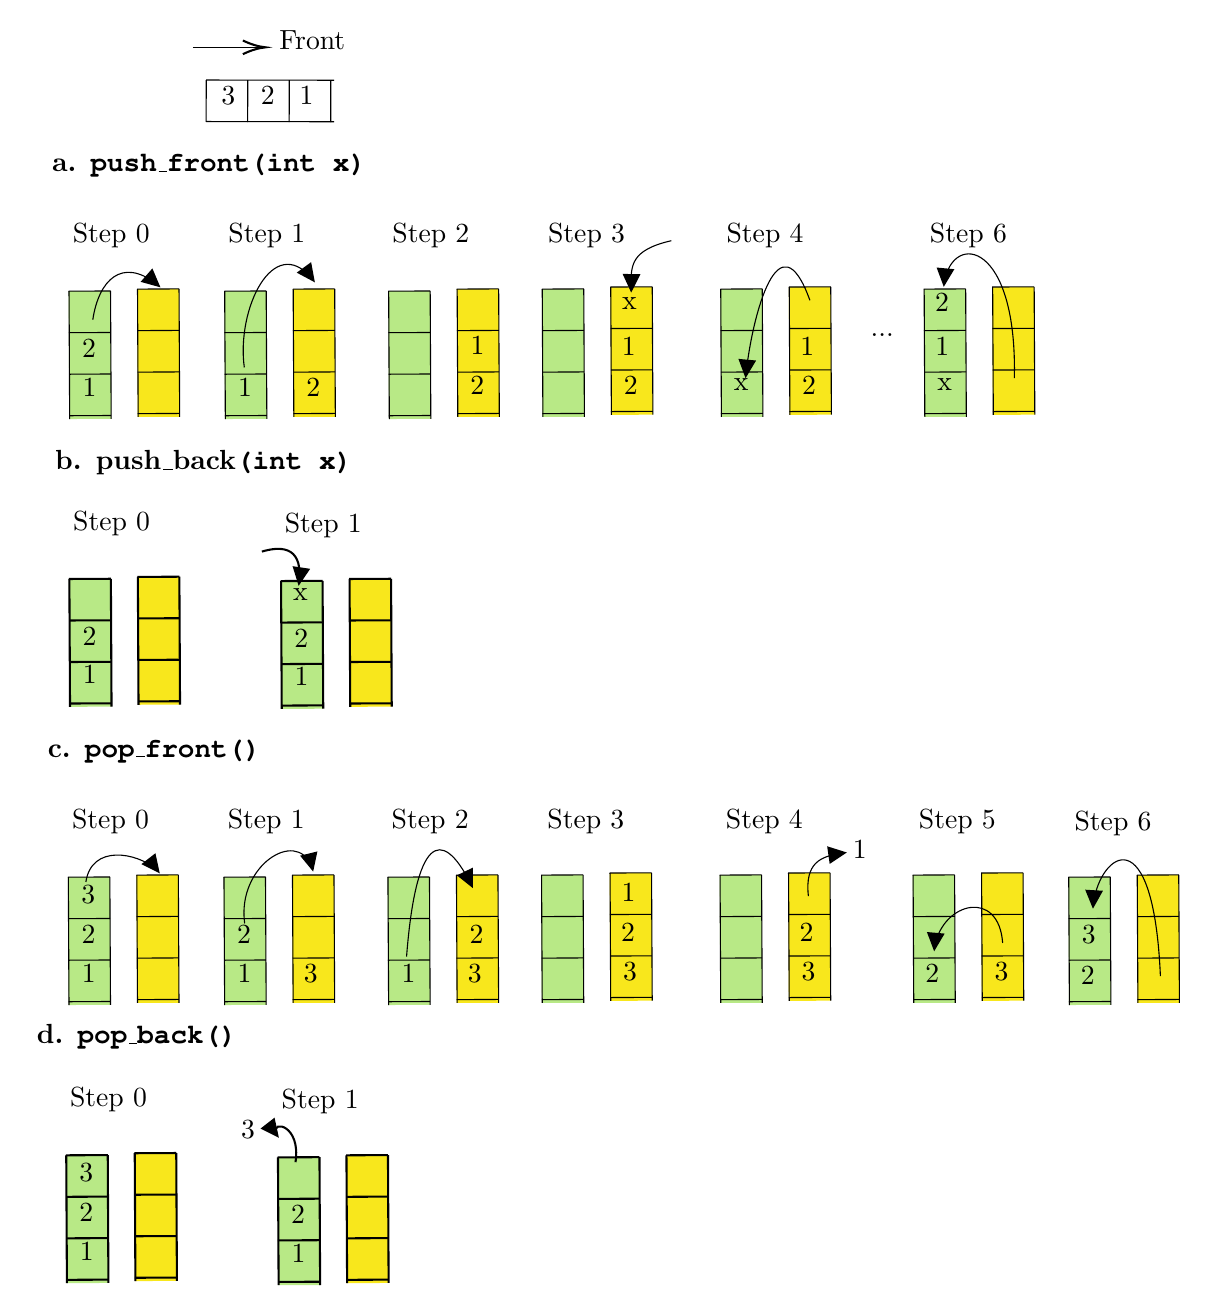
\begin{tikzpicture}[x=0.75pt,y=0.75pt,yscale=-1,xscale=1]
%uncomment if require: \path (0,629); %set diagram left start at 0, and has height of 629

%Shape: Grid [id:dp896547263001342] 
\draw  [draw opacity=0][fill={rgb, 255:red, 184; green, 233; blue, 134 }  ,fill opacity=1 ] (65.74,421.25) -- (66.06,482.85) -- (45.86,482.95) -- (45.54,421.35) -- cycle ; \draw   (65.74,421.25) -- (45.54,421.35)(65.85,441.25) -- (45.65,441.35)(65.95,461.25) -- (45.75,461.35)(66.05,481.25) -- (45.85,481.35) ; \draw   (65.74,421.25) -- (66.06,482.85)(45.74,421.35) -- (46.06,482.95) ; \draw    ;
%Shape: Grid [id:dp865132759524764] 
\draw  [draw opacity=0][fill={rgb, 255:red, 248; green, 231; blue, 28 }  ,fill opacity=1 ] (98.74,420.25) -- (99.06,481.85) -- (78.86,481.95) -- (78.54,420.35) -- cycle ; \draw   (98.74,420.25) -- (78.54,420.35)(98.85,440.25) -- (78.65,440.35)(98.95,460.25) -- (78.75,460.35)(99.05,480.25) -- (78.85,480.35) ; \draw   (98.74,420.25) -- (99.06,481.85)(78.74,420.35) -- (79.06,481.95) ; \draw    ;
%Curve Lines [id:da5103957328612907] 
\draw    (54.2,423.65) .. controls (56.96,405.25) and (78.85,409.58) .. (87.78,417.39) ;
\draw [shift={(89.8,419.5)}, rotate = 232.13] [fill={rgb, 255:red, 0; green, 0; blue, 0 }  ][line width=0.08]  [draw opacity=0] (8.93,-4.29) -- (0,0) -- (8.93,4.29) -- cycle    ;
%Shape: Grid [id:dp10793426839818987] 
\draw  [draw opacity=0][fill={rgb, 255:red, 184; green, 233; blue, 134 }  ,fill opacity=1 ] (293.74,420.25) -- (294.06,481.85) -- (273.86,481.95) -- (273.54,420.35) -- cycle ; \draw   (293.74,420.25) -- (273.54,420.35)(293.85,440.25) -- (273.65,440.35)(293.95,460.25) -- (273.75,460.35)(294.05,480.25) -- (273.85,480.35) ; \draw   (293.74,420.25) -- (294.06,481.85)(273.74,420.35) -- (274.06,481.95) ; \draw    ;
%Shape: Grid [id:dp7402423790337394] 
\draw  [draw opacity=0][fill={rgb, 255:red, 248; green, 231; blue, 28 }  ,fill opacity=1 ] (326.74,419.25) -- (327.06,480.85) -- (306.86,480.95) -- (306.54,419.35) -- cycle ; \draw   (326.74,419.25) -- (306.54,419.35)(326.85,439.25) -- (306.65,439.35)(326.95,459.25) -- (306.75,459.35)(327.05,479.25) -- (306.85,479.35) ; \draw   (326.74,419.25) -- (327.06,480.85)(306.74,419.35) -- (307.06,480.95) ; \draw    ;
%Shape: Grid [id:dp9226434575741493] 
\draw  [draw opacity=0][fill={rgb, 255:red, 184; green, 233; blue, 134 }  ,fill opacity=1 ] (379.74,420.25) -- (380.06,481.85) -- (359.86,481.95) -- (359.54,420.35) -- cycle ; \draw   (379.74,420.25) -- (359.54,420.35)(379.85,440.25) -- (359.65,440.35)(379.95,460.25) -- (359.75,460.35)(380.05,480.25) -- (359.85,480.35) ; \draw   (379.74,420.25) -- (380.06,481.85)(359.74,420.35) -- (360.06,481.95) ; \draw    ;
%Shape: Grid [id:dp2571715192881079] 
\draw  [draw opacity=0][fill={rgb, 255:red, 248; green, 231; blue, 28 }  ,fill opacity=1 ] (412.74,419.25) -- (413.06,480.85) -- (392.86,480.95) -- (392.54,419.35) -- cycle ; \draw   (412.74,419.25) -- (392.54,419.35)(412.85,439.25) -- (392.65,439.35)(412.95,459.25) -- (392.75,459.35)(413.05,479.25) -- (392.85,479.35) ; \draw   (412.74,419.25) -- (413.06,480.85)(392.74,419.35) -- (393.06,480.95) ; \draw    ;
%Curve Lines [id:da1971787957549751] 
\draw    (402.3,430.45) .. controls (400.48,414.07) and (408.6,411.35) .. (417.99,409.87) ;
\draw [shift={(420.8,409.45)}, rotate = 531.87] [fill={rgb, 255:red, 0; green, 0; blue, 0 }  ][line width=0.08]  [draw opacity=0] (8.93,-4.29) -- (0,0) -- (8.93,4.29) -- cycle    ;
%Shape: Grid [id:dp7971310316339648] 
\draw  [draw opacity=0][fill={rgb, 255:red, 184; green, 233; blue, 134 }  ,fill opacity=1 ] (140.74,421.25) -- (141.06,482.85) -- (120.86,482.95) -- (120.54,421.35) -- cycle ; \draw   (140.74,421.25) -- (120.54,421.35)(140.85,441.25) -- (120.65,441.35)(140.95,461.25) -- (120.75,461.35)(141.05,481.25) -- (120.85,481.35) ; \draw   (140.74,421.25) -- (141.06,482.85)(120.74,421.35) -- (121.06,482.95) ; \draw    ;
%Shape: Grid [id:dp5157744262310024] 
\draw  [draw opacity=0][fill={rgb, 255:red, 248; green, 231; blue, 28 }  ,fill opacity=1 ] (173.74,420.25) -- (174.06,481.85) -- (153.86,481.95) -- (153.54,420.35) -- cycle ; \draw   (173.74,420.25) -- (153.54,420.35)(173.85,440.25) -- (153.65,440.35)(173.95,460.25) -- (153.75,460.35)(174.05,480.25) -- (153.85,480.35) ; \draw   (173.74,420.25) -- (174.06,481.85)(153.74,420.35) -- (154.06,481.95) ; \draw    ;
%Curve Lines [id:da957462994857244] 
\draw    (130.7,443.65) .. controls (126.88,415.95) and (155.44,397.84) .. (162.81,415.86) ;
\draw [shift={(163.7,418.65)}, rotate = 256.26] [fill={rgb, 255:red, 0; green, 0; blue, 0 }  ][line width=0.08]  [draw opacity=0] (8.93,-4.29) -- (0,0) -- (8.93,4.29) -- cycle    ;
%Shape: Grid [id:dp7796154872073111] 
\draw  [draw opacity=0][fill={rgb, 255:red, 184; green, 233; blue, 134 }  ,fill opacity=1 ] (219.74,421.25) -- (220.06,482.85) -- (199.86,482.95) -- (199.54,421.35) -- cycle ; \draw   (219.74,421.25) -- (199.54,421.35)(219.85,441.25) -- (199.65,441.35)(219.95,461.25) -- (199.75,461.35)(220.05,481.25) -- (199.85,481.35) ; \draw   (219.74,421.25) -- (220.06,482.85)(199.74,421.35) -- (200.06,482.95) ; \draw    ;
%Shape: Grid [id:dp5298736939102897] 
\draw  [draw opacity=0][fill={rgb, 255:red, 248; green, 231; blue, 28 }  ,fill opacity=1 ] (252.74,420.25) -- (253.06,481.85) -- (232.86,481.95) -- (232.54,420.35) -- cycle ; \draw   (252.74,420.25) -- (232.54,420.35)(252.85,440.25) -- (232.65,440.35)(252.95,460.25) -- (232.75,460.35)(253.05,480.25) -- (232.85,480.35) ; \draw   (252.74,420.25) -- (253.06,481.85)(232.74,420.35) -- (233.06,481.95) ; \draw    ;
%Curve Lines [id:da37974335301226225] 
\draw    (208.7,459.65) .. controls (213.09,403.1) and (225.08,395.98) .. (239.58,424.39) ;
\draw [shift={(240.7,426.65)}, rotate = 244.18] [fill={rgb, 255:red, 0; green, 0; blue, 0 }  ][line width=0.08]  [draw opacity=0] (8.93,-4.29) -- (0,0) -- (8.93,4.29) -- cycle    ;
%Shape: Grid [id:dp06724226085802032] 
\draw  [draw opacity=0][fill={rgb, 255:red, 184; green, 233; blue, 134 }  ,fill opacity=1 ] (472.74,420.25) -- (473.06,481.85) -- (452.86,481.95) -- (452.54,420.35) -- cycle ; \draw   (472.74,420.25) -- (452.54,420.35)(472.85,440.25) -- (452.65,440.35)(472.95,460.25) -- (452.75,460.35)(473.05,480.25) -- (452.85,480.35) ; \draw   (472.74,420.25) -- (473.06,481.85)(452.74,420.35) -- (453.06,481.95) ; \draw    ;
%Shape: Grid [id:dp9253600374291335] 
\draw  [draw opacity=0][fill={rgb, 255:red, 248; green, 231; blue, 28 }  ,fill opacity=1 ] (505.74,419.25) -- (506.06,480.85) -- (485.86,480.95) -- (485.54,419.35) -- cycle ; \draw   (505.74,419.25) -- (485.54,419.35)(505.85,439.25) -- (485.65,439.35)(505.95,459.25) -- (485.75,459.35)(506.05,479.25) -- (485.85,479.35) ; \draw   (505.74,419.25) -- (506.06,480.85)(485.74,419.35) -- (486.06,480.95) ; \draw    ;
%Curve Lines [id:da7081144194020124] 
\draw    (463.33,454.04) .. controls (467.46,433.36) and (493.99,426.79) .. (495.9,453.05) ;
\draw [shift={(462.9,457.05)}, rotate = 274.97] [fill={rgb, 255:red, 0; green, 0; blue, 0 }  ][line width=0.08]  [draw opacity=0] (8.93,-4.29) -- (0,0) -- (8.93,4.29) -- cycle    ;
%Shape: Grid [id:dp6451507790664881] 
\draw  [draw opacity=0][fill={rgb, 255:red, 184; green, 233; blue, 134 }  ,fill opacity=1 ] (547.74,421.25) -- (548.06,482.85) -- (527.86,482.95) -- (527.54,421.35) -- cycle ; \draw   (547.74,421.25) -- (527.54,421.35)(547.85,441.25) -- (527.65,441.35)(547.95,461.25) -- (527.75,461.35)(548.05,481.25) -- (527.85,481.35) ; \draw   (547.74,421.25) -- (548.06,482.85)(527.74,421.35) -- (528.06,482.95) ; \draw    ;
%Shape: Grid [id:dp87814914464261] 
\draw  [draw opacity=0][fill={rgb, 255:red, 248; green, 231; blue, 28 }  ,fill opacity=1 ] (580.74,420.25) -- (581.06,481.85) -- (560.86,481.95) -- (560.54,420.35) -- cycle ; \draw   (580.74,420.25) -- (560.54,420.35)(580.85,440.25) -- (560.65,440.35)(580.95,460.25) -- (560.75,460.35)(581.05,480.25) -- (560.85,480.35) ; \draw   (580.74,420.25) -- (581.06,481.85)(560.74,420.35) -- (561.06,481.95) ; \draw    ;
%Curve Lines [id:da30612195083967286] 
\draw    (539.7,433.56) .. controls (543.06,409.84) and (568.54,391.29) .. (571.9,469.05) ;
\draw [shift={(539.4,436.55)}, rotate = 273.43] [fill={rgb, 255:red, 0; green, 0; blue, 0 }  ][line width=0.08]  [draw opacity=0] (8.93,-4.29) -- (0,0) -- (8.93,4.29) -- cycle    ;
%Shape: Grid [id:dp769602343734243] 
\draw  [draw opacity=0][fill={rgb, 255:red, 184; green, 233; blue, 134 }  ,fill opacity=1 ][line width=0.75]  (64.74,555.25) -- (65.06,616.85) -- (44.86,616.95) -- (44.54,555.35) -- cycle ; \draw  [line width=0.75]  (64.74,555.25) -- (44.54,555.35)(64.85,575.25) -- (44.65,575.35)(64.95,595.25) -- (44.75,595.35)(65.05,615.25) -- (44.85,615.35) ; \draw  [line width=0.75]  (64.74,555.25) -- (65.06,616.85)(44.74,555.35) -- (45.06,616.95) ; \draw  [line width=0.75]   ;
%Shape: Grid [id:dp044067323242499734] 
\draw  [draw opacity=0][fill={rgb, 255:red, 248; green, 231; blue, 28 }  ,fill opacity=1 ][line width=0.75]  (97.74,554.25) -- (98.06,615.85) -- (77.86,615.95) -- (77.54,554.35) -- cycle ; \draw  [line width=0.75]  (97.74,554.25) -- (77.54,554.35)(97.85,574.25) -- (77.65,574.35)(97.95,594.25) -- (77.75,594.35)(98.05,614.25) -- (77.85,614.35) ; \draw  [line width=0.75]  (97.74,554.25) -- (98.06,615.85)(77.74,554.35) -- (78.06,615.95) ; \draw  [line width=0.75]   ;
%Shape: Grid [id:dp47312590077848093] 
\draw  [draw opacity=0][fill={rgb, 255:red, 184; green, 233; blue, 134 }  ,fill opacity=1 ][line width=0.75]  (166.74,556.25) -- (167.06,617.85) -- (146.86,617.95) -- (146.54,556.35) -- cycle ; \draw  [line width=0.75]  (166.74,556.25) -- (146.54,556.35)(166.85,576.25) -- (146.65,576.35)(166.95,596.25) -- (146.75,596.35)(167.05,616.25) -- (146.85,616.35) ; \draw  [line width=0.75]  (166.74,556.25) -- (167.06,617.85)(146.74,556.35) -- (147.06,617.95) ; \draw  [line width=0.75]   ;
%Shape: Grid [id:dp013140850242420177] 
\draw  [draw opacity=0][fill={rgb, 255:red, 248; green, 231; blue, 28 }  ,fill opacity=1 ][line width=0.75]  (199.74,555.25) -- (200.06,616.85) -- (179.86,616.95) -- (179.54,555.35) -- cycle ; \draw  [line width=0.75]  (199.74,555.25) -- (179.54,555.35)(199.85,575.25) -- (179.65,575.35)(199.95,595.25) -- (179.75,595.35)(200.05,615.25) -- (179.85,615.35) ; \draw  [line width=0.75]  (199.74,555.25) -- (200.06,616.85)(179.74,555.35) -- (180.06,616.95) ; \draw  [line width=0.75]   ;
%Curve Lines [id:da6711960814723812] 
\draw [line width=0.75]    (155.2,558.65) .. controls (157.88,540.75) and (143.75,538.27) .. (145.77,544.4) ;
\draw [shift={(147.2,546.9)}, rotate = 232.13] [fill={rgb, 255:red, 0; green, 0; blue, 0 }  ][line width=0.08]  [draw opacity=0] (8.93,-4.29) -- (0,0) -- (8.93,4.29) -- cycle    ;


%Shape: Grid [id:dp016566714249388603] 
\draw  [draw opacity=0][fill={rgb, 255:red, 184; green, 233; blue, 134 }  ,fill opacity=1 ] (66.08,138.92) -- (66.39,200.52) -- (46.19,200.62) -- (45.88,139.02) -- cycle ; \draw   (66.08,138.92) -- (45.88,139.02)(66.18,158.92) -- (45.98,159.02)(66.28,178.92) -- (46.08,179.02)(66.38,198.92) -- (46.18,199.02) ; \draw   (66.08,138.92) -- (66.39,200.52)(46.08,139.02) -- (46.39,200.62) ; \draw    ;
%Shape: Grid [id:dp047078691278701124] 
\draw  [draw opacity=0][fill={rgb, 255:red, 248; green, 231; blue, 28 }  ,fill opacity=1 ] (99.08,137.92) -- (99.39,199.52) -- (79.19,199.62) -- (78.88,138.02) -- cycle ; \draw   (99.08,137.92) -- (78.88,138.02)(99.18,157.92) -- (78.98,158.02)(99.28,177.92) -- (79.08,178.02)(99.38,197.92) -- (79.18,198.02) ; \draw   (99.08,137.92) -- (99.39,199.52)(79.08,138.02) -- (79.39,199.62) ; \draw    ;
%Curve Lines [id:da49034016845329353] 
\draw    (57.53,152.77) .. controls (60.41,133.57) and (71.59,122.66) .. (88.05,135.44) ;
\draw [shift={(90.13,137.17)}, rotate = 221.19] [fill={rgb, 255:red, 0; green, 0; blue, 0 }  ][line width=0.08]  [draw opacity=0] (8.93,-4.29) -- (0,0) -- (8.93,4.29) -- cycle    ;
%Shape: Grid [id:dp642268757278023] 
\draw  [draw opacity=0][fill={rgb, 255:red, 184; green, 233; blue, 134 }  ,fill opacity=1 ] (294.08,137.92) -- (294.39,199.52) -- (274.19,199.62) -- (273.88,138.02) -- cycle ; \draw   (294.08,137.92) -- (273.88,138.02)(294.18,157.92) -- (273.98,158.02)(294.28,177.92) -- (274.08,178.02)(294.38,197.92) -- (274.18,198.02) ; \draw   (294.08,137.92) -- (294.39,199.52)(274.08,138.02) -- (274.39,199.62) ; \draw    ;
%Shape: Grid [id:dp4661804059189958] 
\draw  [draw opacity=0][fill={rgb, 255:red, 248; green, 231; blue, 28 }  ,fill opacity=1 ] (327.08,136.92) -- (327.39,198.52) -- (307.19,198.62) -- (306.88,137.02) -- cycle ; \draw   (327.08,136.92) -- (306.88,137.02)(327.18,156.92) -- (306.98,157.02)(327.28,176.92) -- (307.08,177.02)(327.38,196.92) -- (307.18,197.02) ; \draw   (327.08,136.92) -- (327.39,198.52)(307.08,137.02) -- (307.39,198.62) ; \draw    ;
%Shape: Grid [id:dp34126585925965336] 
\draw  [draw opacity=0][fill={rgb, 255:red, 184; green, 233; blue, 134 }  ,fill opacity=1 ] (380.08,137.92) -- (380.39,199.52) -- (360.19,199.62) -- (359.88,138.02) -- cycle ; \draw   (380.08,137.92) -- (359.88,138.02)(380.18,157.92) -- (359.98,158.02)(380.28,177.92) -- (360.08,178.02)(380.38,197.92) -- (360.18,198.02) ; \draw   (380.08,137.92) -- (380.39,199.52)(360.08,138.02) -- (360.39,199.62) ; \draw    ;
%Shape: Grid [id:dp7902806896116741] 
\draw  [draw opacity=0][fill={rgb, 255:red, 248; green, 231; blue, 28 }  ,fill opacity=1 ] (413.08,136.92) -- (413.39,198.52) -- (393.19,198.62) -- (392.88,137.02) -- cycle ; \draw   (413.08,136.92) -- (392.88,137.02)(413.18,156.92) -- (392.98,157.02)(413.28,176.92) -- (393.08,177.02)(413.38,196.92) -- (393.18,197.02) ; \draw   (413.08,136.92) -- (413.39,198.52)(393.08,137.02) -- (393.39,198.62) ; \draw    ;
%Shape: Grid [id:dp9549655213090111] 
\draw  [draw opacity=0][fill={rgb, 255:red, 184; green, 233; blue, 134 }  ,fill opacity=1 ] (141.08,138.92) -- (141.39,200.52) -- (121.19,200.62) -- (120.88,139.02) -- cycle ; \draw   (141.08,138.92) -- (120.88,139.02)(141.18,158.92) -- (120.98,159.02)(141.28,178.92) -- (121.08,179.02)(141.38,198.92) -- (121.18,199.02) ; \draw   (141.08,138.92) -- (141.39,200.52)(121.08,139.02) -- (121.39,200.62) ; \draw    ;
%Shape: Grid [id:dp297997885614242] 
\draw  [draw opacity=0][fill={rgb, 255:red, 248; green, 231; blue, 28 }  ,fill opacity=1 ] (174.08,137.92) -- (174.39,199.52) -- (154.19,199.62) -- (153.88,138.02) -- cycle ; \draw   (174.08,137.92) -- (153.88,138.02)(174.18,157.92) -- (153.98,158.02)(174.28,177.92) -- (154.08,178.02)(174.38,197.92) -- (154.18,198.02) ; \draw   (174.08,137.92) -- (174.39,199.52)(154.08,138.02) -- (154.39,199.62) ; \draw    ;
%Curve Lines [id:da25833689890539646] 
\draw    (130.53,175.77) .. controls (126.65,147.64) and (144.41,111.04) .. (162.82,132.6) ;
\draw [shift={(164.53,134.77)}, rotate = 233.84] [fill={rgb, 255:red, 0; green, 0; blue, 0 }  ][line width=0.08]  [draw opacity=0] (8.93,-4.29) -- (0,0) -- (8.93,4.29) -- cycle    ;
%Shape: Grid [id:dp9824219895159405] 
\draw  [draw opacity=0][fill={rgb, 255:red, 184; green, 233; blue, 134 }  ,fill opacity=1 ] (220.08,138.92) -- (220.39,200.52) -- (200.19,200.62) -- (199.88,139.02) -- cycle ; \draw   (220.08,138.92) -- (199.88,139.02)(220.18,158.92) -- (199.98,159.02)(220.28,178.92) -- (200.08,179.02)(220.38,198.92) -- (200.18,199.02) ; \draw   (220.08,138.92) -- (220.39,200.52)(200.08,139.02) -- (200.39,200.62) ; \draw    ;
%Shape: Grid [id:dp8389163535925388] 
\draw  [draw opacity=0][fill={rgb, 255:red, 248; green, 231; blue, 28 }  ,fill opacity=1 ] (253.08,137.92) -- (253.39,199.52) -- (233.19,199.62) -- (232.88,138.02) -- cycle ; \draw   (253.08,137.92) -- (232.88,138.02)(253.18,157.92) -- (232.98,158.02)(253.28,177.92) -- (233.08,178.02)(253.38,197.92) -- (233.18,198.02) ; \draw   (253.08,137.92) -- (253.39,199.52)(233.08,138.02) -- (233.39,199.62) ; \draw    ;
%Curve Lines [id:da6804249898768449] 
\draw    (336.27,114.7) .. controls (316.25,119.25) and (316.81,127.13) .. (316.93,136.78) ;
\draw [shift={(316.93,139.7)}, rotate = 270.99] [fill={rgb, 255:red, 0; green, 0; blue, 0 }  ][line width=0.08]  [draw opacity=0] (8.93,-4.29) -- (0,0) -- (8.93,4.29) -- cycle    ;
%Curve Lines [id:da9104687654892889] 
\draw    (403.03,143.42) .. controls (388.08,101.92) and (375.45,150.29) .. (372.33,177.99) ;
\draw [shift={(372.03,180.92)}, rotate = 275.29] [fill={rgb, 255:red, 0; green, 0; blue, 0 }  ][line width=0.08]  [draw opacity=0] (8.93,-4.29) -- (0,0) -- (8.93,4.29) -- cycle    ;
%Shape: Grid [id:dp600821598861303] 
\draw  [draw opacity=0][fill={rgb, 255:red, 184; green, 233; blue, 134 }  ,fill opacity=1 ] (478.08,137.92) -- (478.39,199.52) -- (458.19,199.62) -- (457.88,138.02) -- cycle ; \draw   (478.08,137.92) -- (457.88,138.02)(478.18,157.92) -- (457.98,158.02)(478.28,177.92) -- (458.08,178.02)(478.38,197.92) -- (458.18,198.02) ; \draw   (478.08,137.92) -- (478.39,199.52)(458.08,138.02) -- (458.39,199.62) ; \draw    ;
%Shape: Grid [id:dp9493102449319921] 
\draw  [draw opacity=0][fill={rgb, 255:red, 248; green, 231; blue, 28 }  ,fill opacity=1 ] (511.08,136.92) -- (511.39,198.52) -- (491.19,198.62) -- (490.88,137.02) -- cycle ; \draw   (511.08,136.92) -- (490.88,137.02)(511.18,156.92) -- (490.98,157.02)(511.28,176.92) -- (491.08,177.02)(511.38,196.92) -- (491.18,197.02) ; \draw   (511.08,136.92) -- (511.39,198.52)(491.08,137.02) -- (491.39,198.62) ; \draw    ;
%Curve Lines [id:da8937690919350911] 
\draw    (501.53,180.92) .. controls (502.98,115.3) and (472.3,110.21) .. (467.91,134.19) ;
\draw [shift={(467.53,136.92)}, rotate = 275.29] [fill={rgb, 255:red, 0; green, 0; blue, 0 }  ][line width=0.08]  [draw opacity=0] (8.93,-4.29) -- (0,0) -- (8.93,4.29) -- cycle    ;

%Shape: Grid [id:dp8150603874477107] 
\draw  [draw opacity=0][fill={rgb, 255:red, 184; green, 233; blue, 134 }  ,fill opacity=1 ][line width=0.75]  (66.24,277.58) -- (66.56,339.18) -- (46.36,339.28) -- (46.04,277.68) -- cycle ; \draw  [line width=0.75]  (66.24,277.58) -- (46.04,277.68)(66.35,297.58) -- (46.15,297.68)(66.45,317.58) -- (46.25,317.68)(66.55,337.58) -- (46.35,337.68) ; \draw  [line width=0.75]  (66.24,277.58) -- (66.56,339.18)(46.24,277.68) -- (46.56,339.28) ; \draw  [line width=0.75]   ;
%Shape: Grid [id:dp2147639435937454] 
\draw  [draw opacity=0][fill={rgb, 255:red, 248; green, 231; blue, 28 }  ,fill opacity=1 ][line width=0.75]  (99.24,276.58) -- (99.56,338.18) -- (79.36,338.28) -- (79.04,276.68) -- cycle ; \draw  [line width=0.75]  (99.24,276.58) -- (79.04,276.68)(99.35,296.58) -- (79.15,296.68)(99.45,316.58) -- (79.25,316.68)(99.55,336.58) -- (79.35,336.68) ; \draw  [line width=0.75]  (99.24,276.58) -- (99.56,338.18)(79.24,276.68) -- (79.56,338.28) ; \draw  [line width=0.75]   ;
%Shape: Grid [id:dp19116065963065187] 
\draw  [draw opacity=0][fill={rgb, 255:red, 184; green, 233; blue, 134 }  ,fill opacity=1 ][line width=0.75]  (168.24,278.58) -- (168.56,340.18) -- (148.36,340.28) -- (148.04,278.68) -- cycle ; \draw  [line width=0.75]  (168.24,278.58) -- (148.04,278.68)(168.35,298.58) -- (148.15,298.68)(168.45,318.58) -- (148.25,318.68)(168.55,338.58) -- (148.35,338.68) ; \draw  [line width=0.75]  (168.24,278.58) -- (168.56,340.18)(148.24,278.68) -- (148.56,340.28) ; \draw  [line width=0.75]   ;
%Shape: Grid [id:dp782264924767575] 
\draw  [draw opacity=0][fill={rgb, 255:red, 248; green, 231; blue, 28 }  ,fill opacity=1 ][line width=0.75]  (201.24,277.58) -- (201.56,339.18) -- (181.36,339.28) -- (181.04,277.68) -- cycle ; \draw  [line width=0.75]  (201.24,277.58) -- (181.04,277.68)(201.35,297.58) -- (181.15,297.68)(201.45,317.58) -- (181.25,317.68)(201.55,337.58) -- (181.35,337.68) ; \draw  [line width=0.75]  (201.24,277.58) -- (201.56,339.18)(181.24,277.68) -- (181.56,339.28) ; \draw  [line width=0.75]   ;
%Curve Lines [id:da5458509265772213] 
\draw [line width=0.75]    (157.06,277.87) .. controls (158.37,261.1) and (147.03,262.12) .. (139,264.48) ;
\draw [shift={(156.7,280.98)}, rotate = 278.53] [fill={rgb, 255:red, 0; green, 0; blue, 0 }  ][line width=0.08]  [draw opacity=0] (8.93,-4.29) -- (0,0) -- (8.93,4.29) -- cycle    ;

%Shape: Grid [id:dp08323580092603566] 
\draw  [draw opacity=0] (112.18,37.29) -- (173.78,37.38) -- (173.75,57.58) -- (112.15,57.49) -- cycle ; \draw   (112.18,37.29) -- (112.15,57.49)(132.18,37.32) -- (132.15,57.52)(152.18,37.35) -- (152.15,57.55)(172.18,37.37) -- (172.15,57.57) ; \draw   (112.18,37.29) -- (173.78,37.38)(112.15,57.29) -- (173.75,57.38) ; \draw    ;
%Straight Lines [id:da1564815575390679] 
\draw    (105.77,21.53) -- (138.77,21.53) ;
\draw [shift={(140.77,21.53)}, rotate = 180] [color={rgb, 255:red, 0; green, 0; blue, 0 }  ][line width=0.75]    (10.93,-3.29) .. controls (6.95,-1.4) and (3.31,-0.3) .. (0,0) .. controls (3.31,0.3) and (6.95,1.4) .. (10.93,3.29)   ;




% Text Node
\draw (146.17,12.33) node [anchor=north west][inner sep=0.75pt]   [align=left] {Front};
% Text Node
\draw (50,596) node [anchor=north west][inner sep=0.75pt]   [align=left] {1};
% Text Node
\draw (49.85,577.35) node [anchor=north west][inner sep=0.75pt]   [align=left] {2};
% Text Node
\draw (49.74,558.35) node [anchor=north west][inner sep=0.75pt]   [align=left] {3};
% Text Node
\draw (71.4,528.75) node   [align=left] {\begin{minipage}[lt]{37.26399169921875pt}\setlength\topsep{0pt}
Step 0
\end{minipage}};
% Text Node
\draw (152,597) node [anchor=north west][inner sep=0.75pt]   [align=left] {1};
% Text Node
\draw (151.85,578.35) node [anchor=north west][inner sep=0.75pt]   [align=left] {2};
% Text Node
\draw (127.74,537.35) node [anchor=north west][inner sep=0.75pt]   [align=left] {3};
% Text Node
\draw (173.4,529.75) node   [align=left] {\begin{minipage}[lt]{37.26399169921875pt}\setlength\topsep{0pt}
Step 1
\end{minipage}};
% Text Node
\draw (89.85,497.99) node   [align=left] {\begin{minipage}[lt]{88.876pt}\setlength\topsep{0pt}
\textbf{d. {\fontfamily{pcr}\selectfont pop\_back()}}
\end{minipage}};
% Text Node
\draw (155.8,39.39) node [anchor=north west][inner sep=0.75pt]  [rotate=-359.54] [align=left] {1};
% Text Node
\draw (118.32,39.3) node [anchor=north west][inner sep=0.75pt]  [rotate=-0.74] [align=left] {3};
% Text Node
\draw (137.22,39.38) node [anchor=north west][inner sep=0.75pt]  [rotate=-0.02] [align=left] {2};
% Text Node
\draw (155.12,77.99) node   [align=left] {\begin{minipage}[lt]{175.82532918294268pt}\setlength\topsep{0pt}
\textbf{a. {\fontfamily{pcr}\selectfont push\_front(int x)}}
\end{minipage}};
% Text Node
\draw (226.73,112.42) node   [align=left] {\begin{minipage}[lt]{37.26399169921875pt}\setlength\topsep{0pt}
Step 2
\end{minipage}};
% Text Node
\draw (238.18,179.02) node [anchor=north west][inner sep=0.75pt]   [align=left] {2};
% Text Node
\draw (238.33,159.67) node [anchor=north west][inner sep=0.75pt]   [align=left] {1};
% Text Node
\draw (147.73,112.42) node   [align=left] {\begin{minipage}[lt]{37.26399169921875pt}\setlength\topsep{0pt}
Step 1
\end{minipage}};
% Text Node
\draw (159.18,180.02) node [anchor=north west][inner sep=0.75pt]   [align=left] {2};
% Text Node
\draw (126.33,179.67) node [anchor=north west][inner sep=0.75pt]   [align=left] {1};
% Text Node
\draw (72.73,112.42) node   [align=left] {\begin{minipage}[lt]{37.26399169921875pt}\setlength\topsep{0pt}
Step 0
\end{minipage}};
% Text Node
\draw (311.33,140.67) node [anchor=north west][inner sep=0.75pt]   [align=left] {x};
% Text Node
\draw (311.18,160.02) node [anchor=north west][inner sep=0.75pt]   [align=left] {1};
% Text Node
\draw (312.08,179.02) node [anchor=north west][inner sep=0.75pt]   [align=left] {2};
% Text Node
\draw (301.73,112.42) node   [align=left] {\begin{minipage}[lt]{37.26399169921875pt}\setlength\topsep{0pt}
Step 3
\end{minipage}};
% Text Node
\draw (397.18,160.02) node [anchor=north west][inner sep=0.75pt]   [align=left] {1};
% Text Node
\draw (398.08,179.02) node [anchor=north west][inner sep=0.75pt]   [align=left] {2};
% Text Node
\draw (387.73,112.42) node   [align=left] {\begin{minipage}[lt]{37.26399169921875pt}\setlength\topsep{0pt}
Step 4
\end{minipage}};
% Text Node
\draw (51.18,161.02) node [anchor=north west][inner sep=0.75pt]   [align=left] {2};
% Text Node
\draw (51.33,179.67) node [anchor=north west][inner sep=0.75pt]   [align=left] {1};
% Text Node
\draw (365.18,180.02) node [anchor=north west][inner sep=0.75pt]   [align=left] {x};
% Text Node
\draw (431.03,158.17) node [anchor=north west][inner sep=0.75pt]   [align=left] {...};
% Text Node
\draw (462.18,160.02) node [anchor=north west][inner sep=0.75pt]   [align=left] {1};
% Text Node
\draw (462.08,139.02) node [anchor=north west][inner sep=0.75pt]   [align=left] {2};
% Text Node
\draw (485.73,112.42) node   [align=left] {\begin{minipage}[lt]{37.26399169921875pt}\setlength\topsep{0pt}
Step 6
\end{minipage}};
% Text Node
\draw (463.18,180.02) node [anchor=north west][inner sep=0.75pt]   [align=left] {x};
% Text Node
\draw (169.2,221.66) node   [align=left] {\begin{minipage}[lt]{194.752pt}\setlength\topsep{0pt}
\textbf{b. push\_back{\fontfamily{pcr}\selectfont (int x)}}
\end{minipage}};
% Text Node
\draw (174.9,252.08) node   [align=left] {\begin{minipage}[lt]{37.26399169921875pt}\setlength\topsep{0pt}
Step 1
\end{minipage}};
% Text Node
\draw (152.74,281.18) node [anchor=north west][inner sep=0.75pt]   [align=left] {x};
% Text Node
\draw (153.35,300.68) node [anchor=north west][inner sep=0.75pt]   [align=left] {2};
% Text Node
\draw (153.5,319.33) node [anchor=north west][inner sep=0.75pt]   [align=left] {1};
% Text Node
\draw (72.9,251.08) node   [align=left] {\begin{minipage}[lt]{37.26399169921875pt}\setlength\topsep{0pt}
Step 0
\end{minipage}};
% Text Node
\draw (51.35,299.68) node [anchor=north west][inner sep=0.75pt]   [align=left] {2};
% Text Node
\draw (51.5,318.33) node [anchor=north west][inner sep=0.75pt]   [align=left] {1};
% Text Node
\draw (136.45,360.32) node   [align=left] {\begin{minipage}[lt]{150.89200000000002pt}\setlength\topsep{0pt}
\textbf{c. {\fontfamily{pcr}\selectfont pop\_front()}}
\end{minipage}};
% Text Node
\draw (51,462) node [anchor=north west][inner sep=0.75pt]   [align=left] {1};
% Text Node
\draw (50.85,443.35) node [anchor=north west][inner sep=0.75pt]   [align=left] {2};
% Text Node
\draw (50.74,424.35) node [anchor=north west][inner sep=0.75pt]   [align=left] {3};
% Text Node
\draw (387.4,394.75) node   [align=left] {\begin{minipage}[lt]{37.26399169921875pt}\setlength\topsep{0pt}
Step 4
\end{minipage}};
% Text Node
\draw (397.74,461.35) node [anchor=north west][inner sep=0.75pt]   [align=left] {3};
% Text Node
\draw (396.85,442.35) node [anchor=north west][inner sep=0.75pt]   [align=left] {2};
% Text Node
\draw (422.5,402.5) node [anchor=north west][inner sep=0.75pt]   [align=left] {1};
% Text Node
\draw (301.4,394.75) node   [align=left] {\begin{minipage}[lt]{37.26399169921875pt}\setlength\topsep{0pt}
Step 3
\end{minipage}};
% Text Node
\draw (311.74,461.35) node [anchor=north west][inner sep=0.75pt]   [align=left] {3};
% Text Node
\draw (310.85,442.35) node [anchor=north west][inner sep=0.75pt]   [align=left] {2};
% Text Node
\draw (311,423) node [anchor=north west][inner sep=0.75pt]   [align=left] {1};
% Text Node
\draw (72.4,394.75) node   [align=left] {\begin{minipage}[lt]{37.26399169921875pt}\setlength\topsep{0pt}
Step 0
\end{minipage}};
% Text Node
\draw (126,462) node [anchor=north west][inner sep=0.75pt]   [align=left] {1};
% Text Node
\draw (125.85,443.35) node [anchor=north west][inner sep=0.75pt]   [align=left] {2};
% Text Node
\draw (157.95,462.35) node [anchor=north west][inner sep=0.75pt]   [align=left] {3};
% Text Node
\draw (147.4,394.75) node   [align=left] {\begin{minipage}[lt]{37.26399169921875pt}\setlength\topsep{0pt}
Step 1
\end{minipage}};
% Text Node
\draw (205,462) node [anchor=north west][inner sep=0.75pt]   [align=left] {1};
% Text Node
\draw (237.85,443.35) node [anchor=north west][inner sep=0.75pt]   [align=left] {2};
% Text Node
\draw (236.95,462.35) node [anchor=north west][inner sep=0.75pt]   [align=left] {3};
% Text Node
\draw (226.4,394.75) node   [align=left] {\begin{minipage}[lt]{37.26399169921875pt}\setlength\topsep{0pt}
Step 2
\end{minipage}};
% Text Node
\draw (480.4,394.75) node   [align=left] {\begin{minipage}[lt]{37.26399169921875pt}\setlength\topsep{0pt}
Step 5
\end{minipage}};
% Text Node
\draw (490.74,461.35) node [anchor=north west][inner sep=0.75pt]   [align=left] {3};
% Text Node
\draw (457.35,462.35) node [anchor=north west][inner sep=0.75pt]   [align=left] {2};
% Text Node
\draw (555.4,395.75) node   [align=left] {\begin{minipage}[lt]{37.26399169921875pt}\setlength\topsep{0pt}
Step 6
\end{minipage}};
% Text Node
\draw (532.85,443.35) node [anchor=north west][inner sep=0.75pt]   [align=left] {3};
% Text Node
\draw (532.35,463.35) node [anchor=north west][inner sep=0.75pt]   [align=left] {2};


\end{tikzpicture}

\item \texttt{push\_front()}: $\textcolor{blue}{O(n^2)-time}$ \par
Pop all elements from the left stack $n$ times, and push all elements, including $x$, back $n+1$ times. Hence, we have $O(n^2)$-time.
\item \texttt{push\_back()}: $\textcolor{blue}{O(1)-time}$ \par
No matter how many elements in the stack are, we only have to push one time. Hecce, $O(1)$-time.
\item \texttt{pop\_front()}: $\textcolor{blue}{O(n^2)-time}$\par
Pop all elements from the left stack $n$ times, push the front element, and then push all elements, including $x$, back $n$ times. Hence, we have $O(n^2)$-time.
\item \texttt{pop\_back()}: $\textcolor{blue}{O(1)-time}$\par
No matter how many elements in the stack are, we only have to pop one time. Hecce, $O(1)$-time.

\item Dynamic stack\par

Assuming $a$ is the size of initial stack, and $q$ is the number of \texttt{enlarge()} calls.
We have $a3^{q}=n$ or $q=\log_{3}(n/a)$. On the other hand, If $t=c_{0}m$ is the time required for single \texttt{enlarge()} calls with $m$ elements, then the total time required for all reallocations is
\begin{equation}
c_{0}a+c_{0}a3^1+c_{0}a3^2+\dots+c_{0}a3^{q-1}=0.5c_{0}a\left(3^{q+1}-1\right)=\Theta(3^{q}).
\label{Dynamic stack}
\end{equation}

Substituting $q=\log_{3}(n/a)$ into Eq.(\ref{Dynamic stack}) yields the time complexity \textcolor{blue}{$\Theta(n)$} required for $n$ consecutive push operations into dynamic stack.
\end{enumerate}


\section*{Problem 3}
\begin{enumerate}
\definecolor{bg}{rgb}{0.95,0.95,0.95}
\item Code:\par
       \begin{minted}
       [
       frame=lines,
       framesep=2mm,
       baselinestretch=1.2,
       bgcolor=bg,
       fontsize=\footnotesize,
       linenos
       ]{c}
         int main(){
         
           int A[6] = {2,0,1,3,4,3}; // The array given by statement
           int i=3;                  // initial position of the frog
           int j=0;                  // counter of loop
           
           while(1){
           
             int next = A[i];
           
             if ( A[i] == i ){
               printf("Frog will stop!\n");
               break;
             }
             else if( j == 6 ){
               printf("Frog will keep jumping forever!\n");
               break;
             }
           
             i = next;
             j++;
           }
           
           return 0;
         
         }
       \end{minted}
         \begin{itemize}
           \item Time complexity is \textcolor{blue}{$\Theta(n)$} since we loop over the array \texttt{A[i]}. If the counter \texttt{j} equals to the length of the array \texttt{A[i]}, then we stop the loop and think the frog will keep jumping forever.
           \item Extra-space complexity is \textcolor{blue}{$\Theta(1)$} because we do not use the helper array to keep track where the frog passes.
         \end{itemize}
         \definecolor{bg}{rgb}{0.95,0.95,0.95}
         \item Code:\par
         \begin{minted}
         [
         frame=lines,
         framesep=2mm,
         baselinestretch=1.2,
         bgcolor=bg,
         fontsize=\footnotesize,
         linenos
         ]{c}
             int main(){
             
               int A[8] = {1,0,4,2,3,1,4,6};   // The array given by statement
               int B[8] = {0};                 // helper array to keep track of where the frog passes
               int i = 2;                      // Initial position of the frog
               int j = 0;                      // loop counter
             
             
             
               while(1){
             
                 if (B[i] != 1){
                   B[i] = 1;
                   j++;
                 }else{
                   printf("The length of the loop is %d\n", j);
                   break;
                 }
             
                 i = A[i];  
               }
             
               return 0;
             }
         \end{minted}
         \begin{itemize}
         \item Time complexity is \textcolor{blue}{$\Theta(n)$} since we loop over the array \texttt{A[i]}. We stop the loop and return the counter \texttt{j} which represent the length of the loop when the helper array \texttt{B[i]} equals to $1$.
         \item Extra-space complexity is \textcolor{blue}{$\Theta(n)$} because the frog may enter the infinite loop from non-initial position, and thus we need the helper array \texttt{B[i]} to keep track where the frog passes.
         \end{itemize}

\item find the minimum of $f(i,j)$\par
         \begin{itemize}
           \item Time complexity is \textcolor{blue}{$\Theta(n)$}.
           \item Extra-space complexity is \textcolor{blue}{$\Theta(1)$}.
         \end{itemize}
         Since the array is strictly increasing, the two indice \texttt{i} and \texttt{j} must be as close as possible
         so that $f(i,j)$ can reach the minimum. i.e. $\texttt{j}=\texttt{i}+1$. Using the constraint $\texttt{j}=\texttt{i}+1$,
         we simply loop the index \texttt{i} over the array and compare the current $f(i,j)$ with the previous one to find
         the minimum $f(i,j)$.
         
\item  Circularly linked list (CLL):\par
    a) Loop over the CLL from the head find the node, say \texttt{A}, having the maximum data.\\
    b) Loop over again the CLL from the node \texttt{A->next} instead of \texttt{A}.\\
    c) During the loop, if the next data is smaller than the current data, we remove the next node from the CLL and store the data in the next node in helper array.
       Note that the size of helper array is expected to be 2 as the CLL only have 2 decreasing.\\
    d) After the second loop, we finally loop over the CLL and insert the data into the proper position.\\
    e) In summary, we loop the CLL 3 times and use one helper array with length 2. Thus, the time complexity is $O(n)$,
       and the extra-space complexity is $O(1)$.

\end{enumerate}

\end{document}
